\documentclass{beamer}
\usepackage[utf8]{inputenc}
\usepackage{graphicx}

\title{Topluluk Tespiti: Klasik Algoritmalar ve Çizge Sinir Ağları Karşılaştırması}
\author{Emre YILDIZ}
\institute{Ege Üniversitesi \\ Bilgisayar Mühendisliği Bölümü}
\date{\today}

\usetheme{Madrid}
\usecolortheme{beaver}

\begin{document}

\begin{frame}
    \titlepage
\end{frame}

\begin{frame}{Proje Hakkında}
    \begin{itemize}
        \item \textbf{Ders:} Cebirsel Çizge Algoritmaları (Yüksek Lisans)
        \item \textbf{Amaç:} Çizge Teorisi'nin teorik temellerini modern Makine Öğrenmesi uygulamaları ile birleştiren kapsamlı bir topluluk tespiti (community detection) çalışmasıdır.
        \item \textbf{Yöntemler:} Neo4j ve PyTorch kullanarak klasik algoritmaları (Louvain, LPA) Graph Neural Networks (GCN, GraphSAGE, GAT) ile karşılaştırmak.
        \item \textbf{Veriseti:} Cora Citation Network.
    \end{itemize}
\end{frame}

\begin{frame}{Kullanılan Kütüphane ve Araçlar}
    \begin{itemize}
        \item \textbf{Neo4j (GDS):} Yüksek performanslı çizge veritabanı. Louvain ve Label Propagation gibi klasik topluluk tespit algoritmalarını çalıştırmak için kullanıldı.
        \item \textbf{PyTorch (PyG):} Derin öğrenme ve özellikle Çizge Sinir Ağları (GNN) modelleri oluşturmak ve eğitmek için kullanılan esnek bir kütüphane.
        \item \textbf{NetworkX:} Çizge oluşturma, manipülasyonu ve temel çizge metriklerinin hesaplanması için kullanıldı.
        \item \textbf{Scikit-learn:} GNN modellerinin performansını değerlendirmek için Adjusted Rand Index (ARI) ve Normalized Mutual Information (NMI) gibi metriklerin hesaplanmasında kullanıldı.
        \item \textbf{Seaborn \& Matplotlib:} Veri ve sonuçların görselleştirilmesi, karşılaştırma grafikleri oluşturulması için kullanıldı.
    \end{itemize}
\end{frame}

\begin{frame}{Klasik Algoritmalar}
    \framesubtitle{Neo4j GDS ile Uygulama}
    \begin{block}{Louvain Algoritması}
        Modülerlik skorunu maksimize ederek toplulukları bulmaya çalışan hiyerarşik bir kümeleme algoritmasıdır. İki aşamadan oluşur:
        \begin{enumerate}
            \item Her düğüm kendi komşularıyla birleştirilerek modülerlik artışı en üst düzeye çıkarılır.
            \item Oluşturulan topluluklar tek bir düğüm olarak kabul edilir ve ilk aşama tekrarlanır.
        \end{enumerate}
    \end{block}
    \begin{block}{Label Propagation Algorithm (LPA)}
        Düğümlerin etiketlerini komşularının en sık rastlanan etiketine göre güncellediği iteratif bir süreçtir. Hızlı ve basittir ancak sonuçları deterministik olmayabilir.
    \end{block}
\end{frame}

\begin{frame}{Graph Neural Network (GNN) Modelleri}
    \framesubtitle{PyTorch Geometric ile Uygulama}
    \begin{block}{Graph Convolutional Network (GCN)}
        Komşu düğümlerin özelliklerini toplayarak ve bir sinir ağı katmanından geçirerek düğüm temsillerini öğrenir. Spektral çizge teorisine dayanır.
    \end{block}
    \begin{block}{GraphSAGE (Sample and Aggregate)}
        Büyük çizgeler için tasarlanmıştır. Her düğüm için komşuluktan sabit sayıda örneklem alır ve bu örneklemlerin bilgilerini birleştirerek (aggregate) düğüm temsilini günceller.
    \end{block}
    \begin{block}{Graph Attention Network (GAT)}
        Komşu düğümlere farklı ağırlıklar atamak için dikkat (attention) mekanizmalarını kullanır. Bu sayede model, hangi komşuların daha önemli olduğuna karar verebilir.
    \end{block}
\end{frame}

\begin{frame}{Sonuçlar: Veriseti İstatistikleri}
    \begin{figure}
        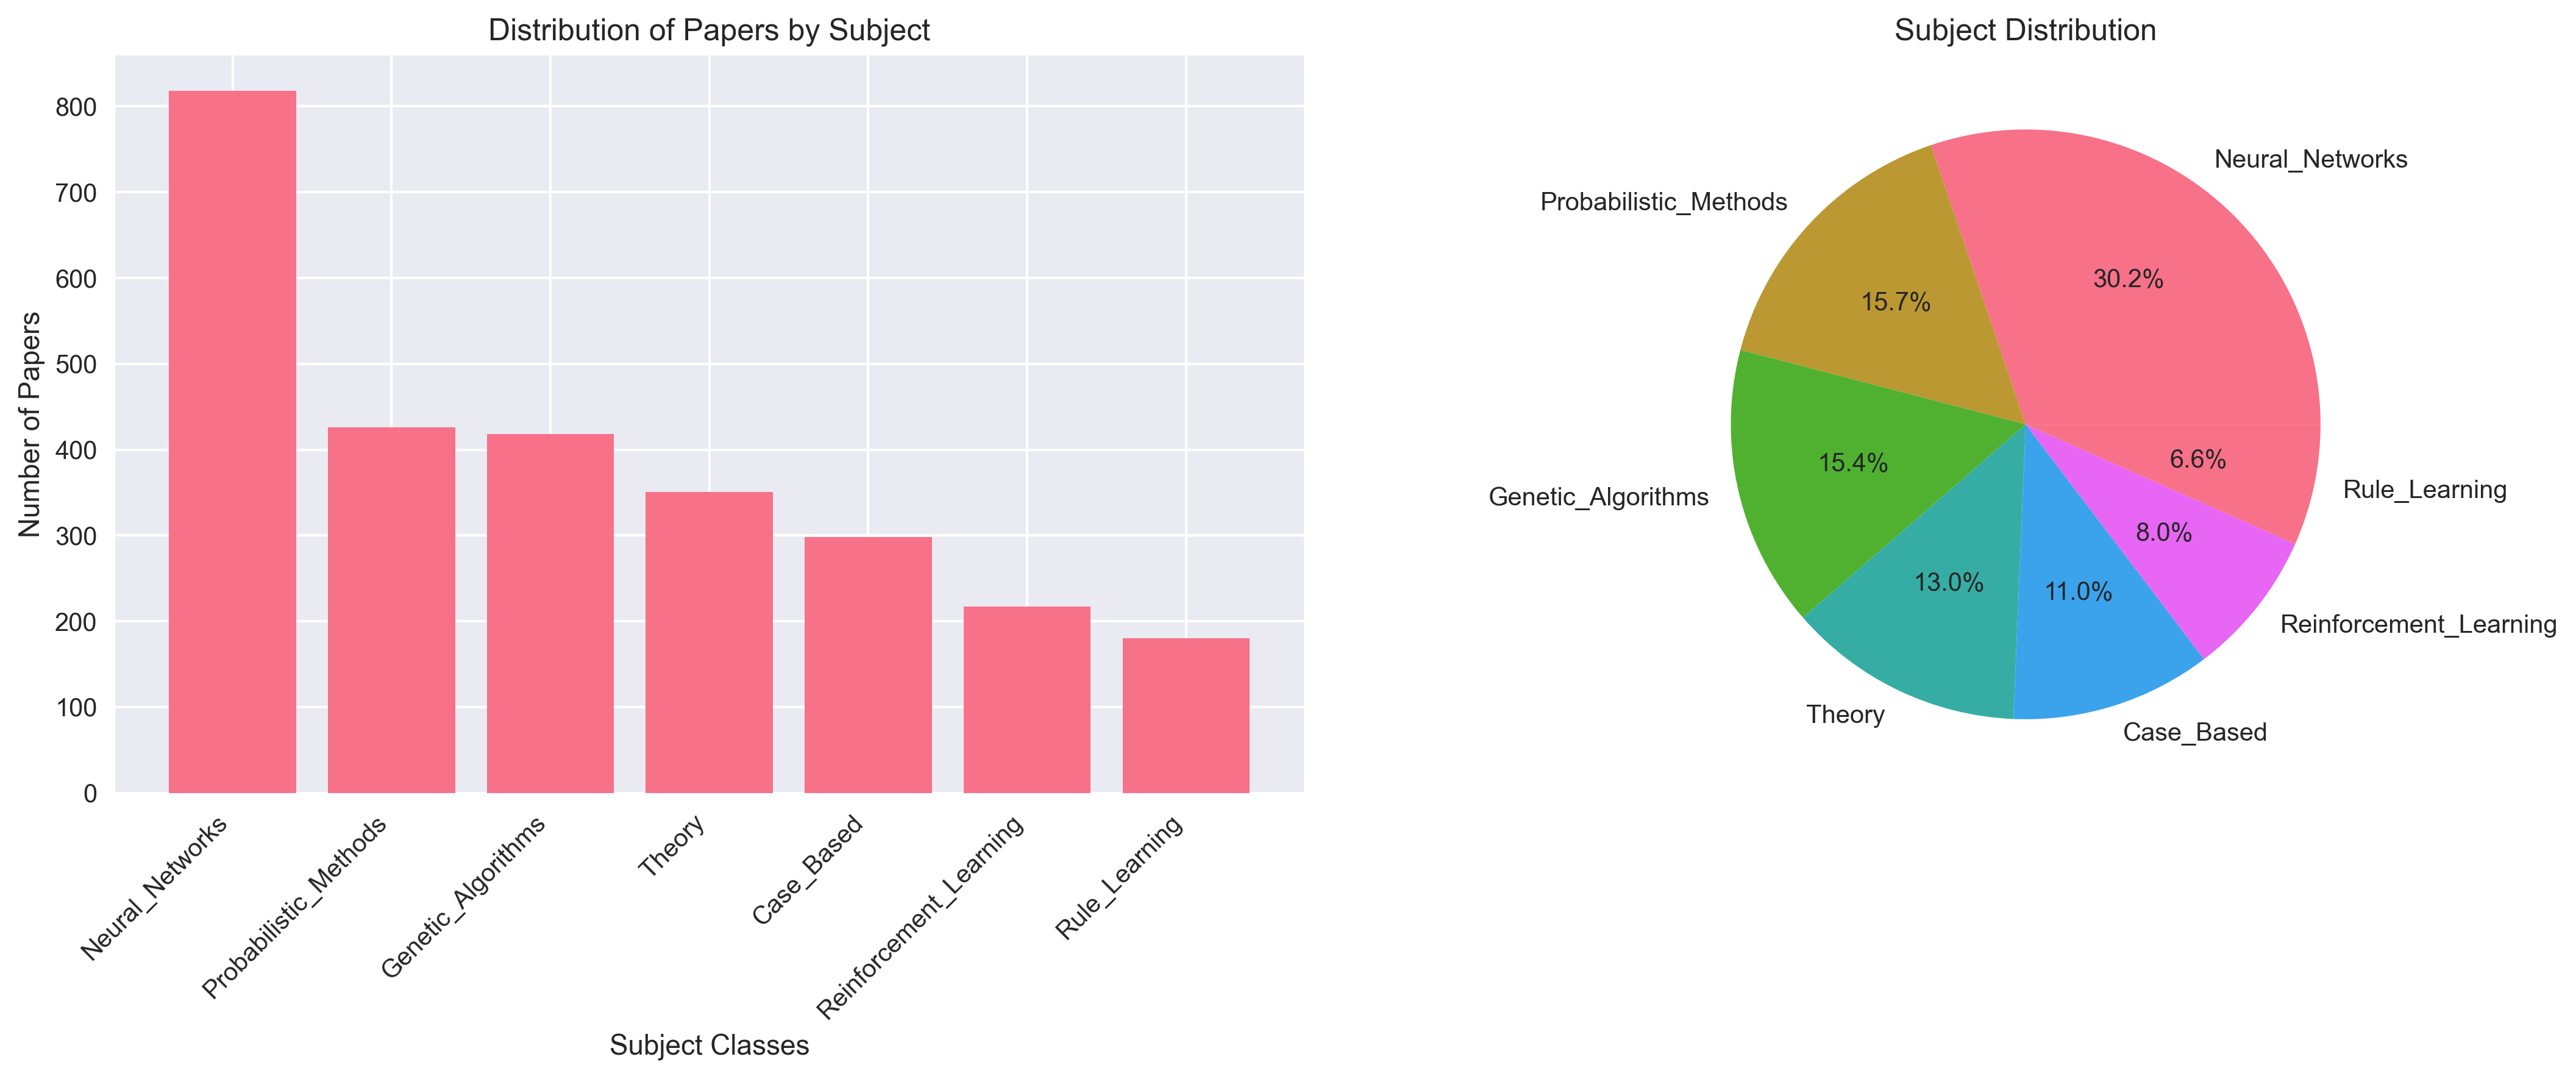
\includegraphics[width=\textwidth]{../results/dataset_stats.png}
        \caption{Cora verisetinin temel istatistikleri ve derece dağılımı.}
    \end{figure}
\end{frame}

\begin{frame}{Sonuçlar: Topluluk Karşılaştırması}
    \begin{figure}
        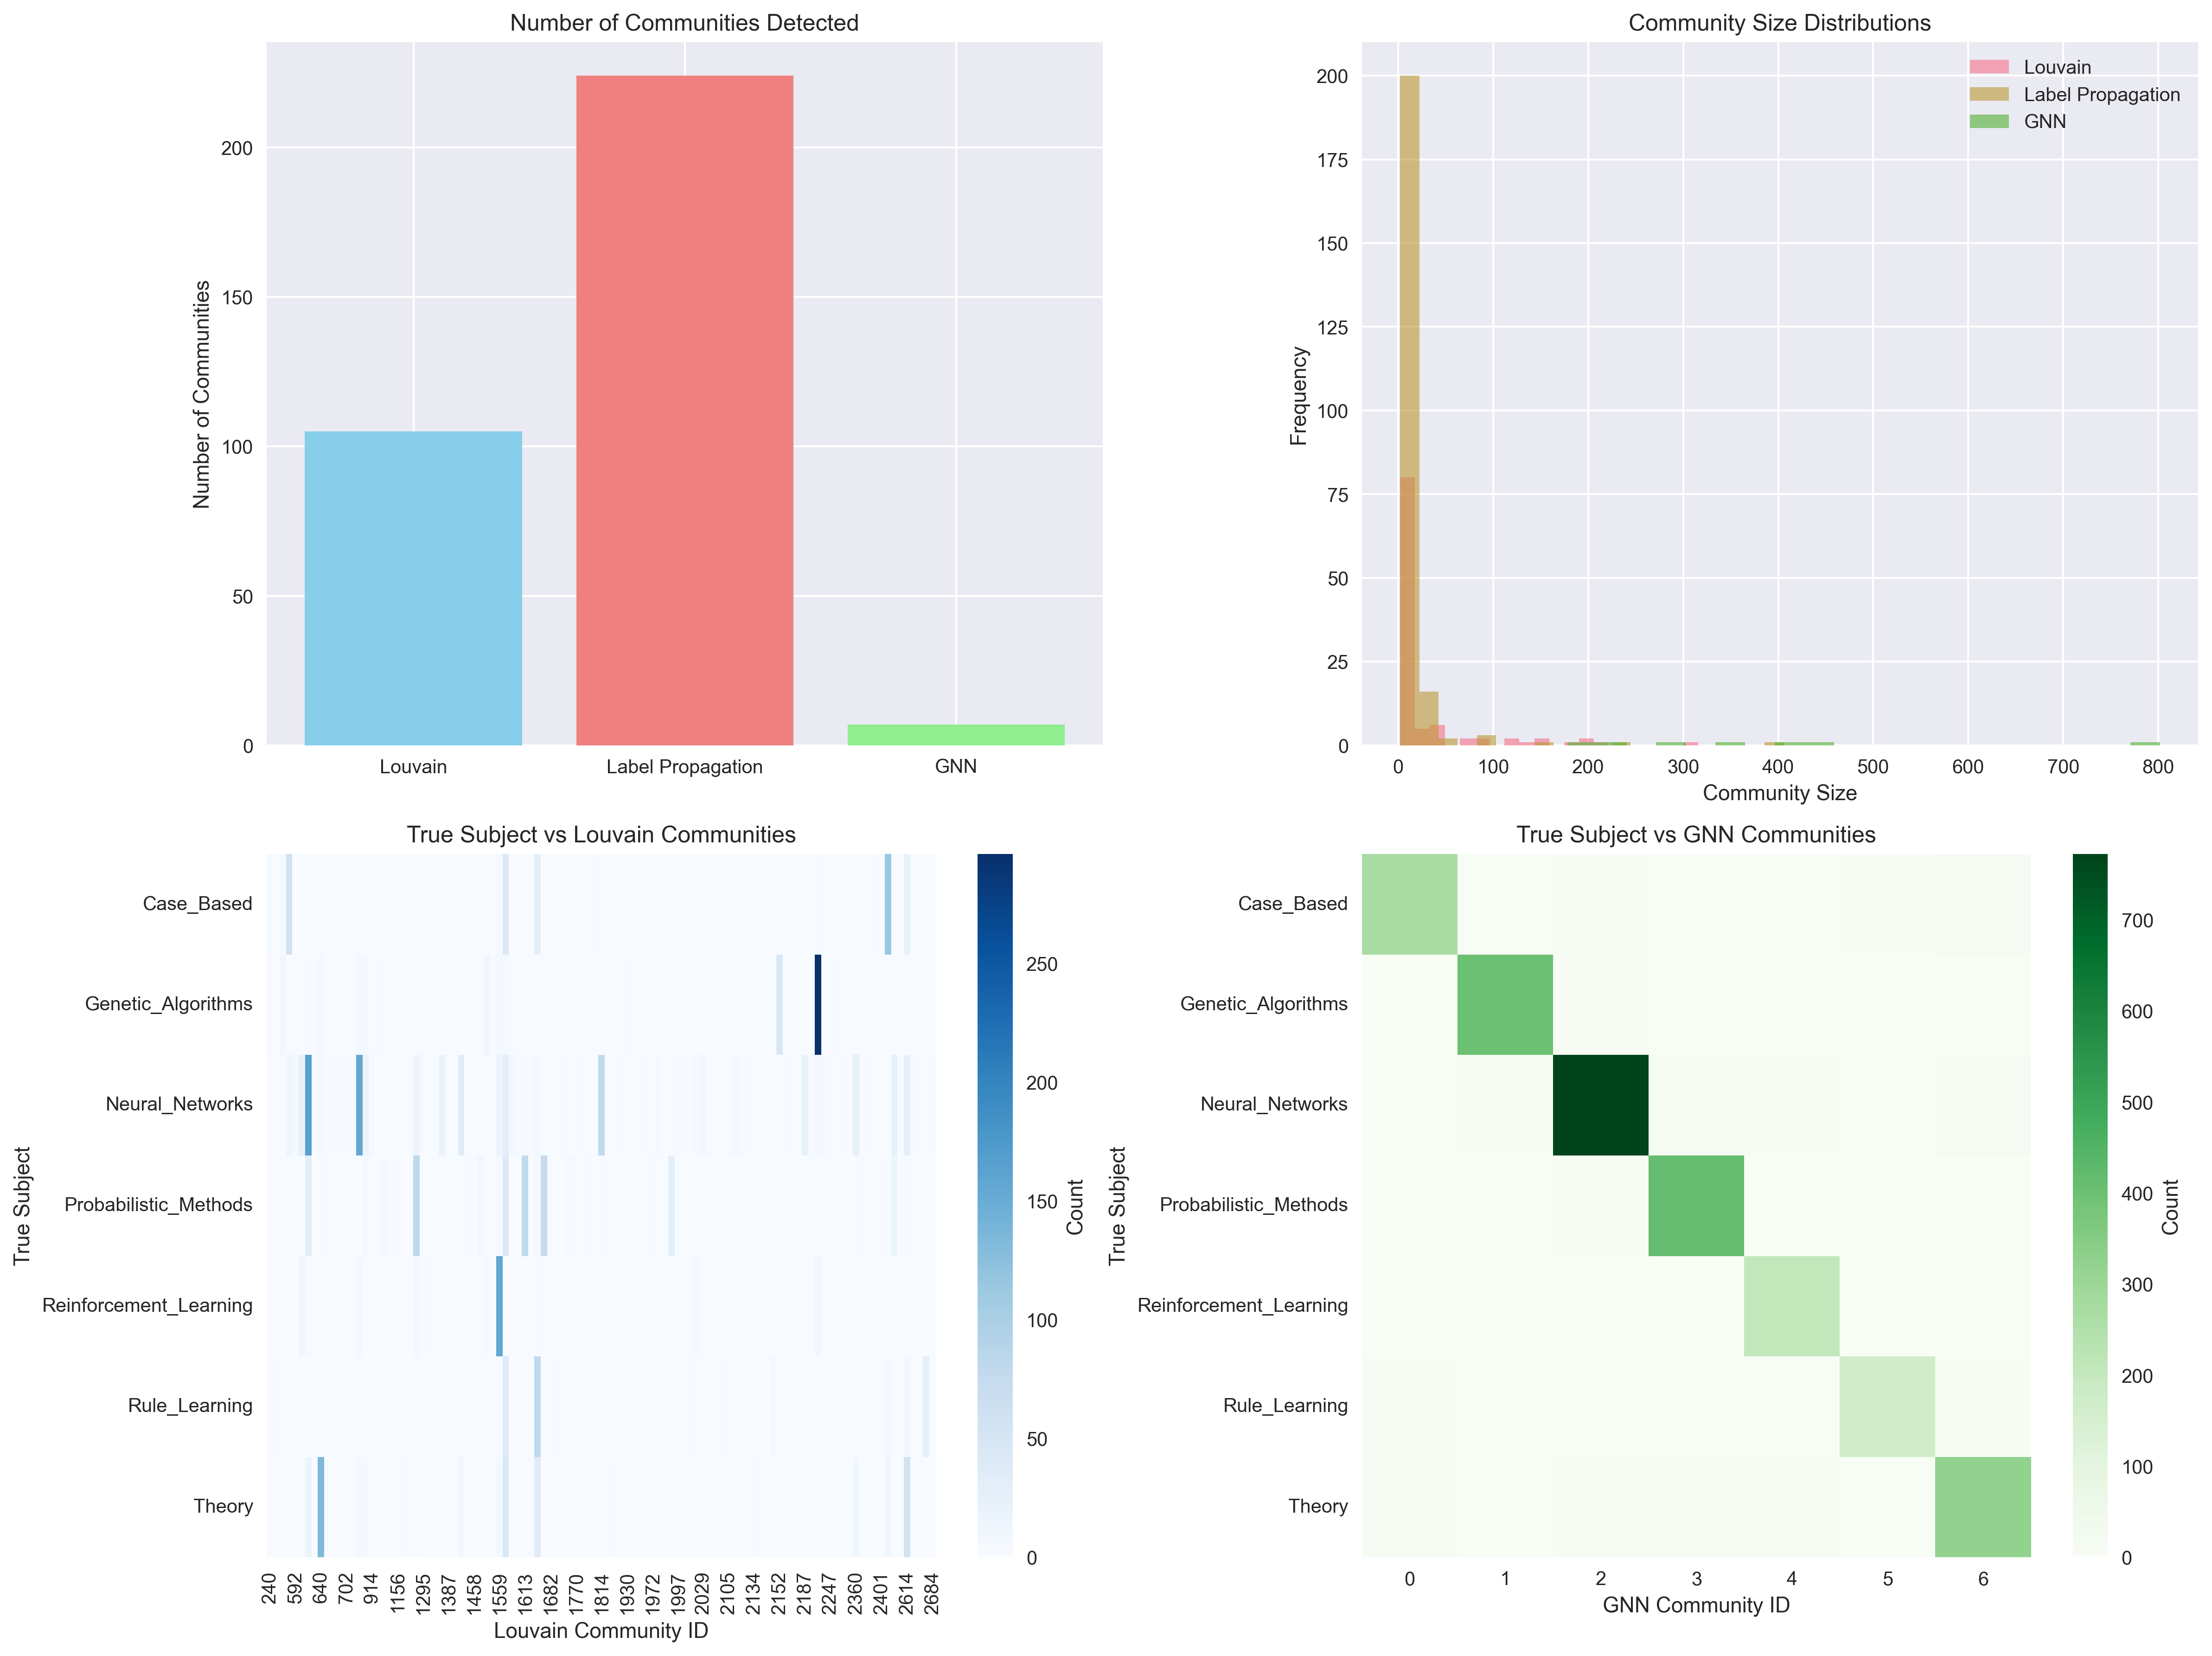
\includegraphics[width=\textwidth]{../results/community_comparison.png}
        \caption{Farklı algoritmalar tarafından tespit edilen topluluk sayılarının karşılaştırması.}
    \end{figure}
\end{frame}

\begin{frame}{Sonuçlar: Değerlendirme Metrikleri}
    \begin{figure}
        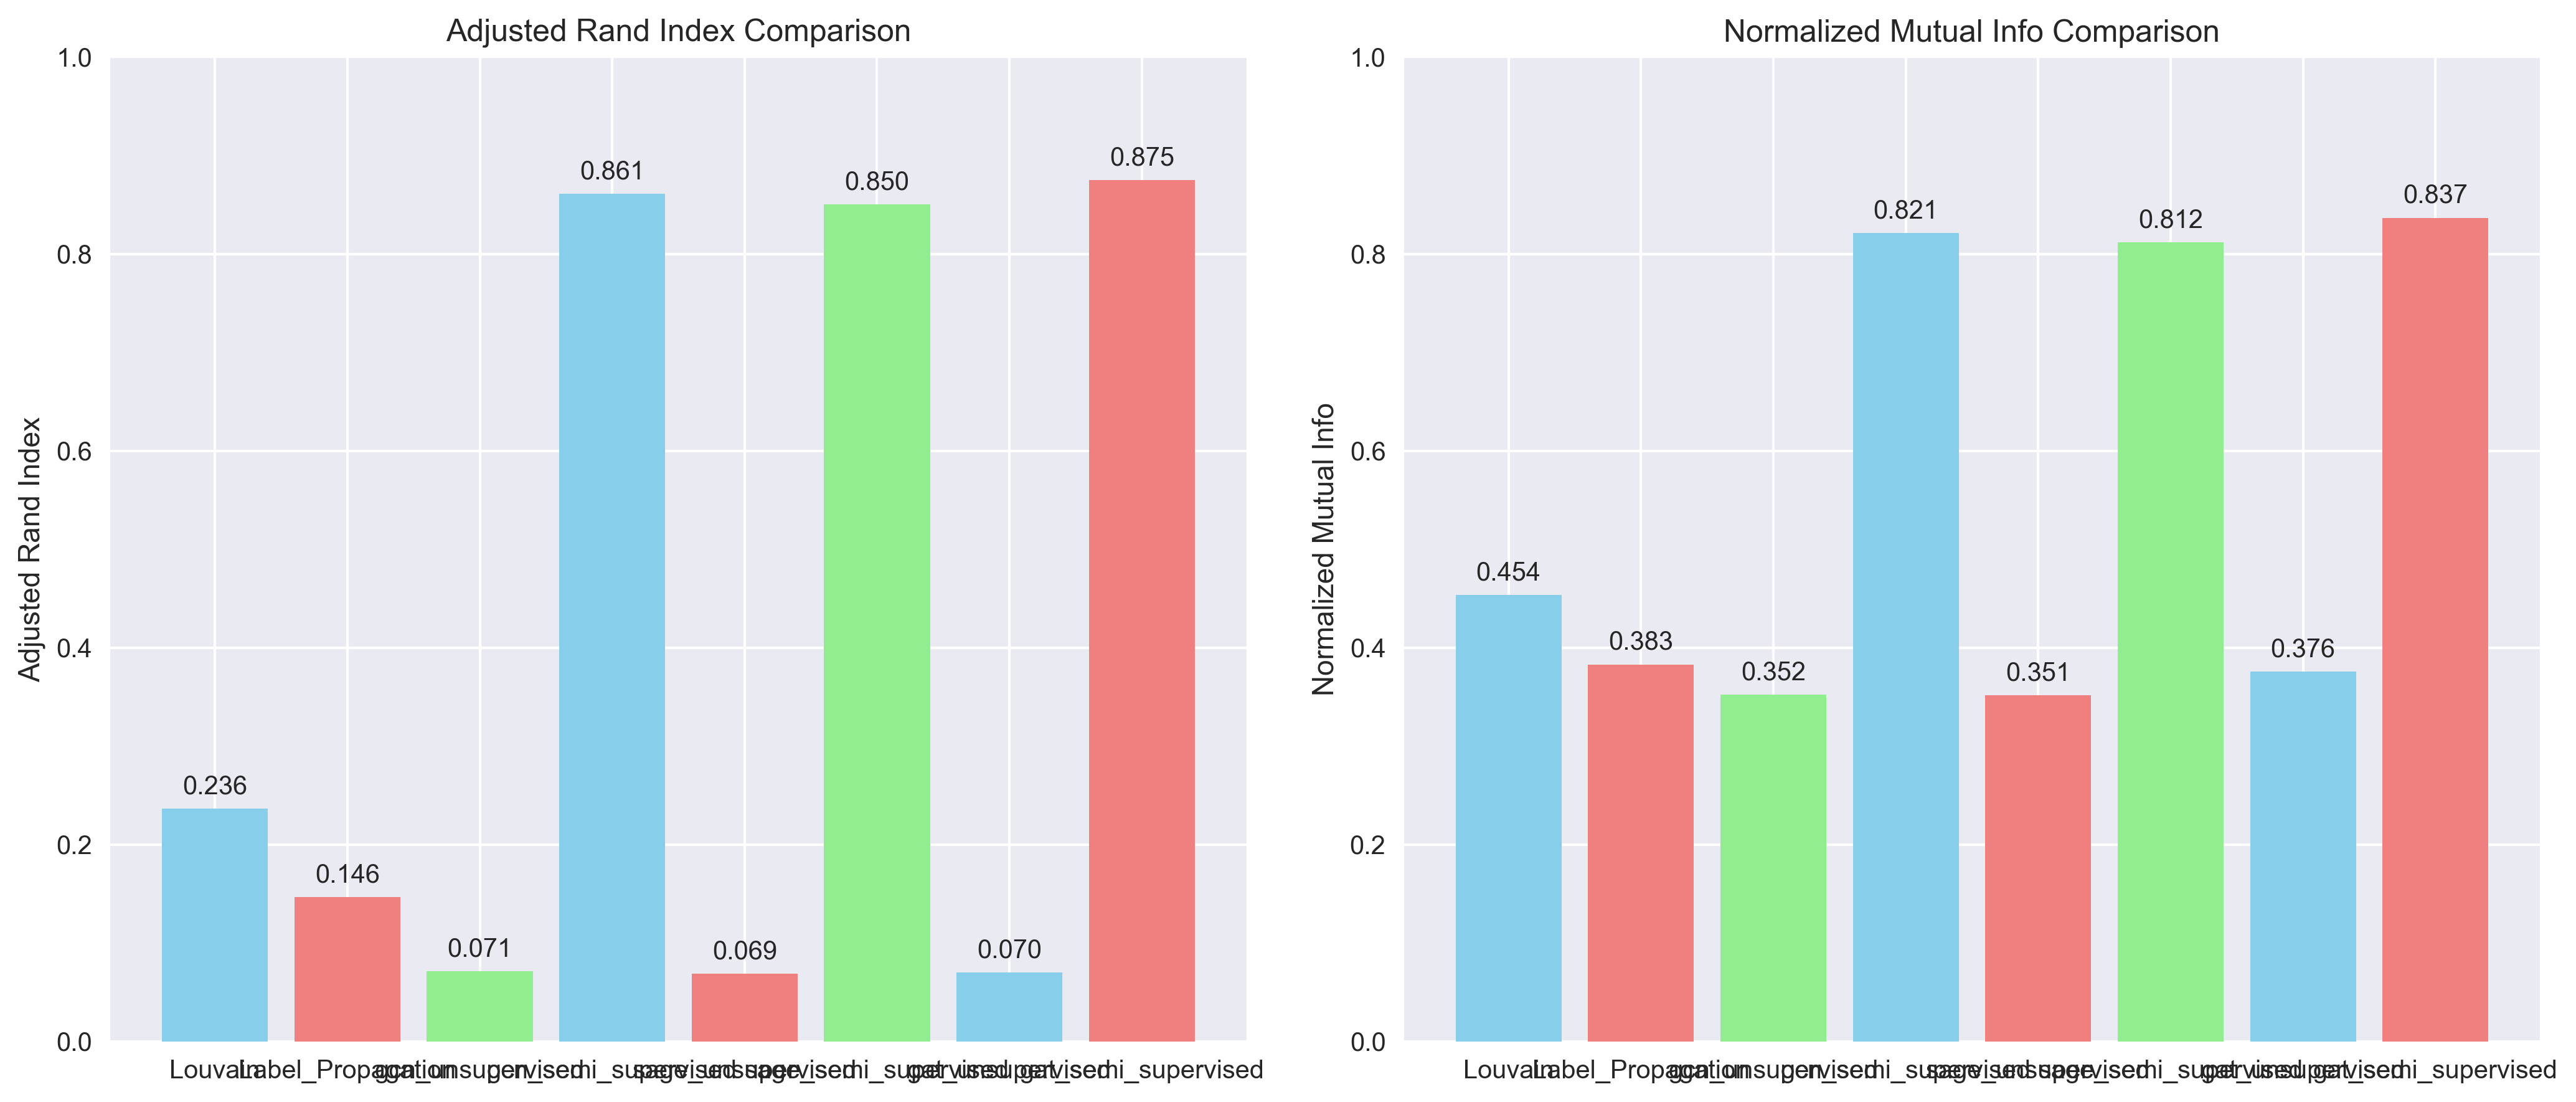
\includegraphics[width=\textwidth]{../results/evaluation_metrics.png}
        \caption{Algoritmaların ARI, NMI ve Modülerlik metriklerine göre performans karşılaştırması.}
    \end{figure}
\end{frame}

\begin{frame}{Sonuçlar: t-SNE ile Düğüm Gösterimi (Figure 1)}
    \begin{figure}
        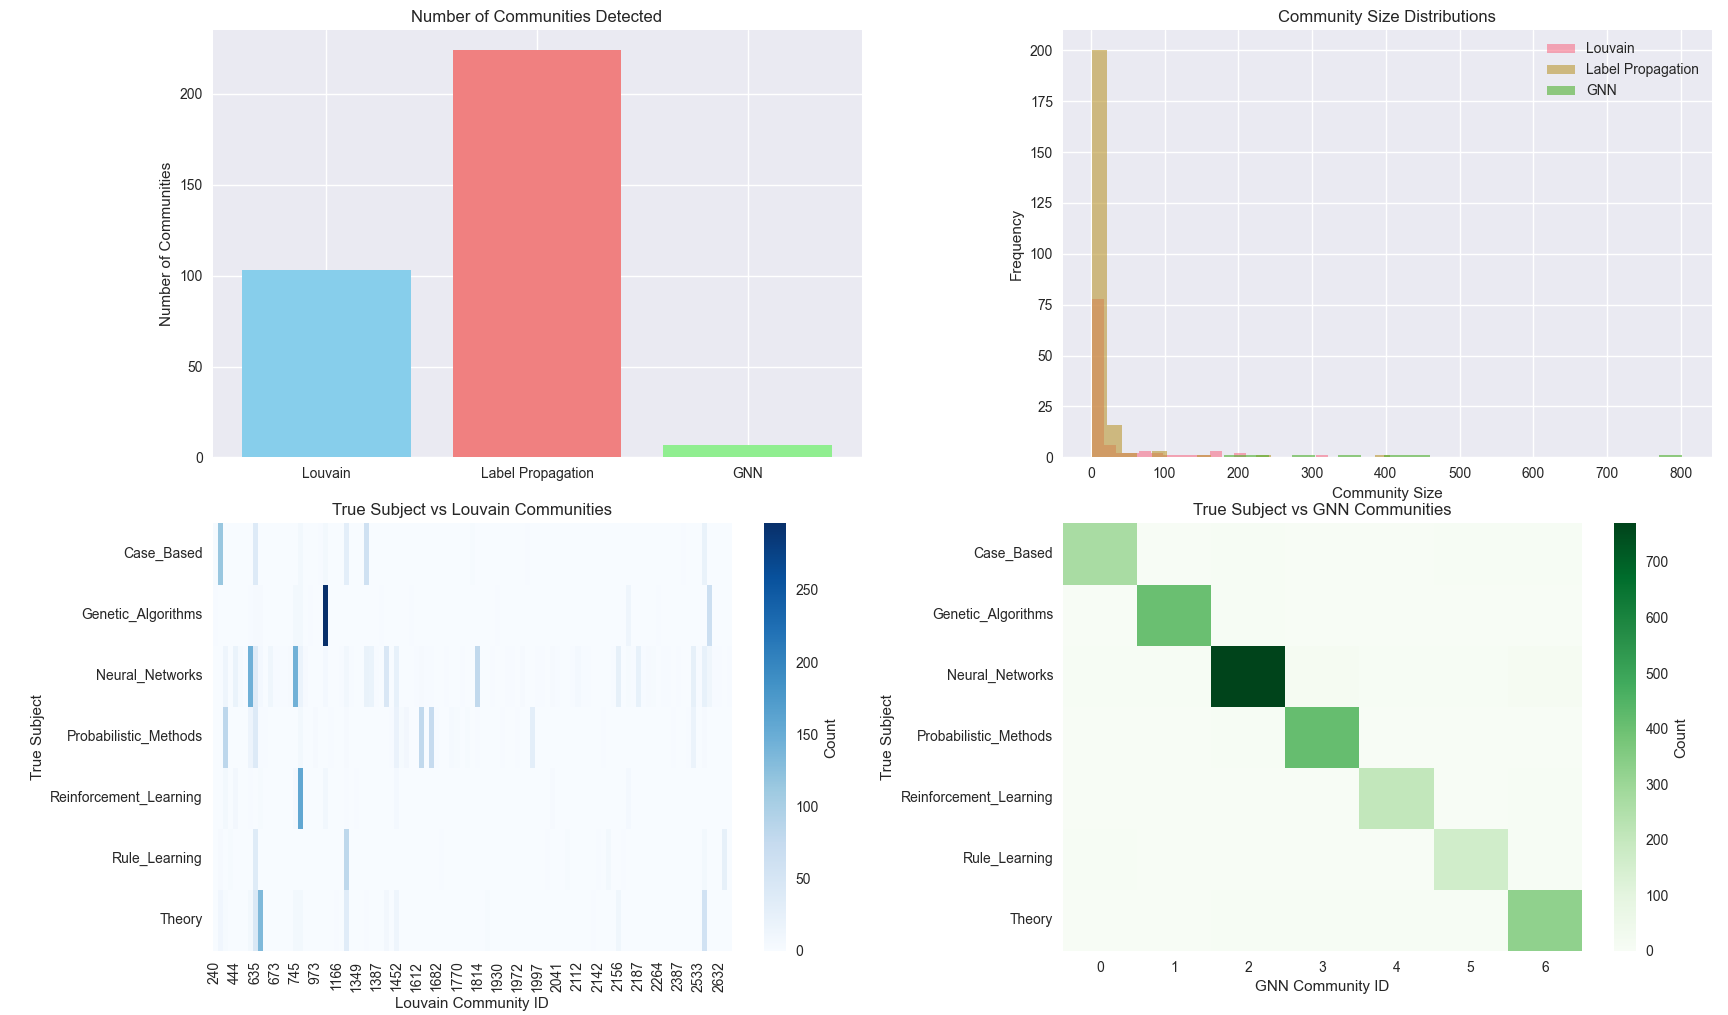
\includegraphics[width=\textwidth]{../results/Figure_1.png}
        \caption{GCN modeli tarafından öğrenilen düğüm gömülmelerinin (embeddings) t-SNE ile 2 boyuta indirgenmiş hali.}
    \end{figure}
\end{frame}

\begin{frame}{Sonuçlar: t-SNE ile Düğüm Gösterimi (Figure 2)}
    \begin{figure}
        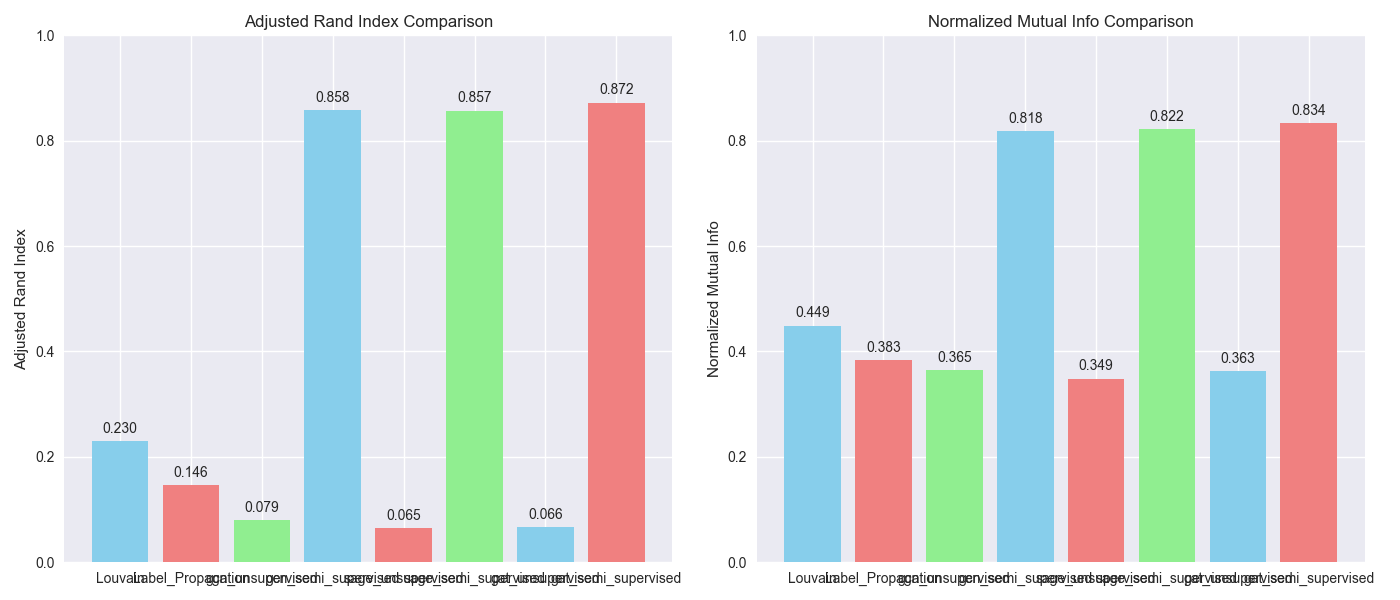
\includegraphics[width=\textwidth]{../results/Figure_2.png}
        \caption{GraphSAGE modeli tarafından öğrenilen düğüm gömülmelerinin (embeddings) t-SNE ile 2 boyuta indirgenmiş hali.}
    \end{figure}
\end{frame}

\begin{frame}{Teşekkürler}
    \centering
    \Huge
    Sorularınız için teşekkür ederim.
\end{frame}

\end{document}
